\chapter{Análise de Resultados}

Nesta secção serão abordadas duas ferramentas de monitorização de tráfego, o \textbf{MRTG} e o \textbf{NTOP}.

\section{MRTG}

\subsection{Configuração}

O \textbf{MRTG} é uma ferramenta capaz de monitorizar o tráfego SNMP numa rede.
Através do MRTG, pode-se monitorizar o tráfego que entra e sai da nossa rede, com a informação apresentada em gráficos com diversos intervalos de tempo.
Deste modo, analisa-se de uma forma visual os padrões de tráfego da nossa rede.

Durante configuração do MRTG \cite{mrtg}, este foi configurado para que analisasse o tráfego no router de bancada (172.16.1.19).
Este router foi configurado de modo a que o serviço SNMP estivesse ativo e o MRTG pudesse obter essa informação.

\subsection{Propriedades da rede} \label{prop_rede}

\begin{figure}
    \centering
    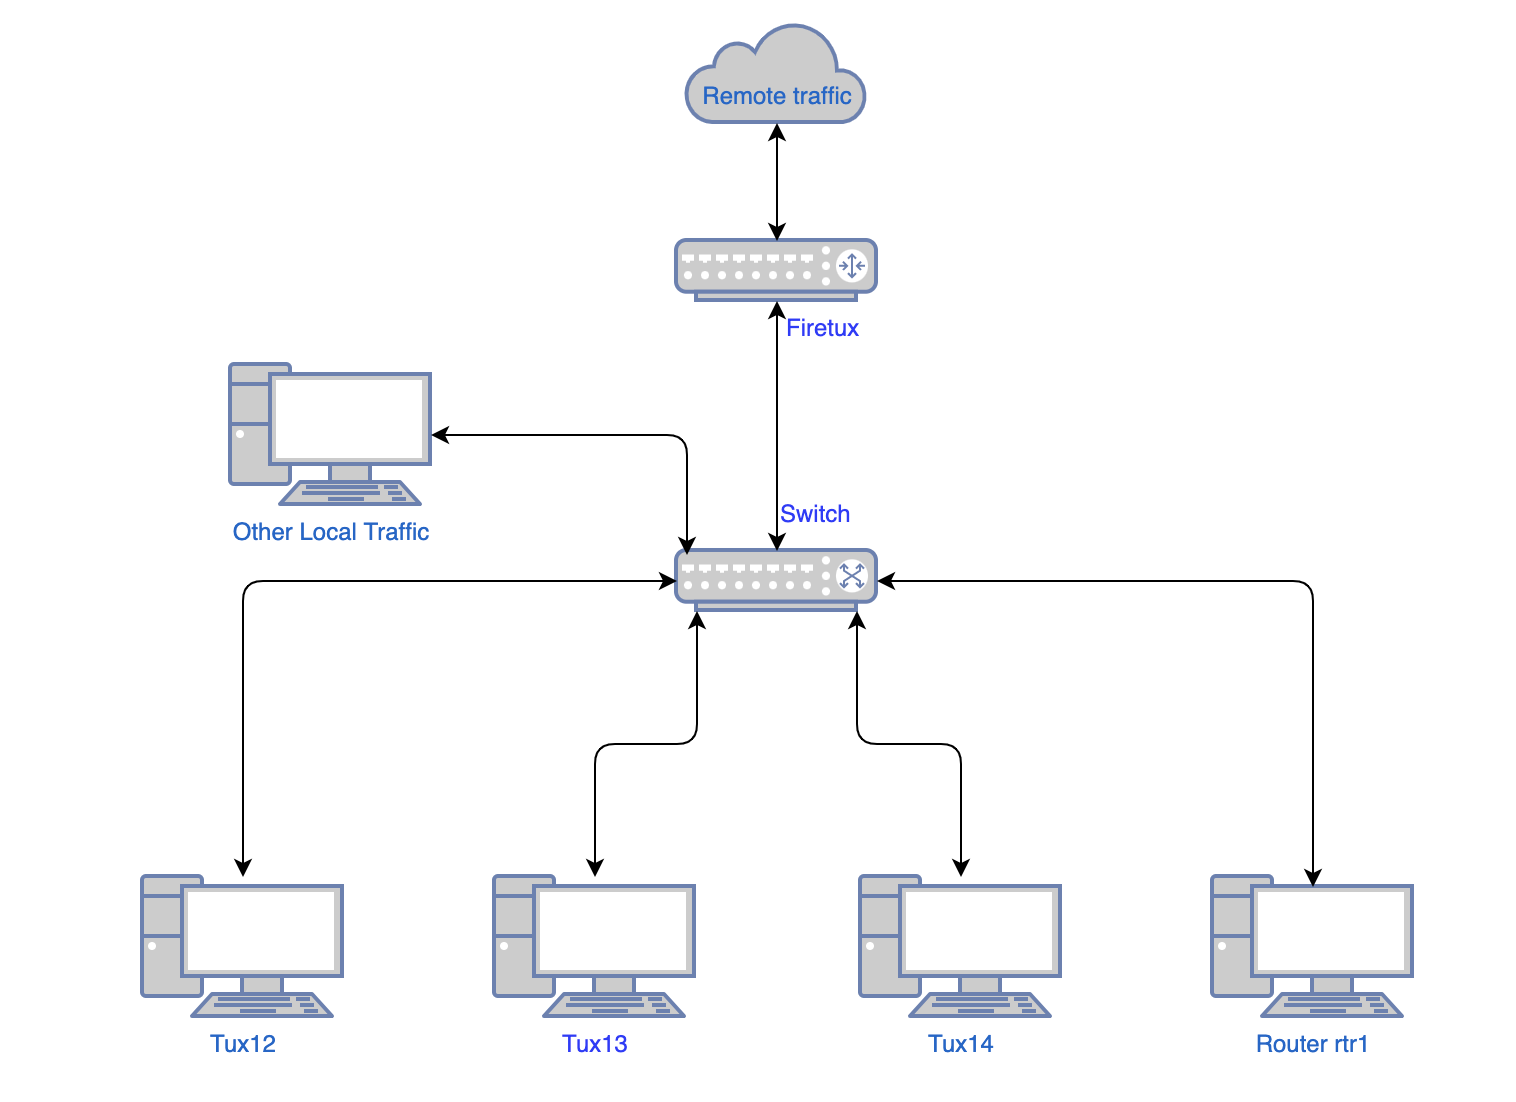
\includegraphics[width=.6\linewidth]{figs/setup/network.png}
    \caption{Configuração da rede neste trabalho}
    \label{fig:network}
\end{figure}

Devido à configuração da rede no laboratório, não é obrigatório que todo o tráfego passe pelo router de bancada (Fig \ref{fig:network}).

Em primeiro lugar, o \textbf{tráfego local} faz uso do \textbf{switch}, logo esse tráfego não será registado pelo MRTG dado que não passa pelo router de bancada.
Isto inclui todo o tráfego entre todos os \textit{tux}s da sala I321.

Em segundo lugar, o router de bancada faz parte da mesma rede local que os \textit{tux}s, ligados pelo switch ao router de sala \textbf{firetux}.
Deste modo, não é obrigatório que um acesso de um tux a um host externo passe pelo router de bancada.
Foi preciso então configurar os \textit{tux}s, de modo a que utilizassem o router de bancada como \textit{default gateway} para forçar o tráfego a ir por esse caminho.
O router de bancada por sua vez tem o router de sala como o seu \textit{default gateway} (Fig \ref{fig:traceroute_1}).
Isto só funciona para novos queries, dado que da segunda vez que fazemos um acesso, o algoritmo irá determinar automaticamente que o melhor caminho é diretamente pelo \textbf{firetux} e mais uma vez o tráfego não irá ser registado (Fig \ref{fig:traceroute_2}).

\begin{figure}
    \centering
    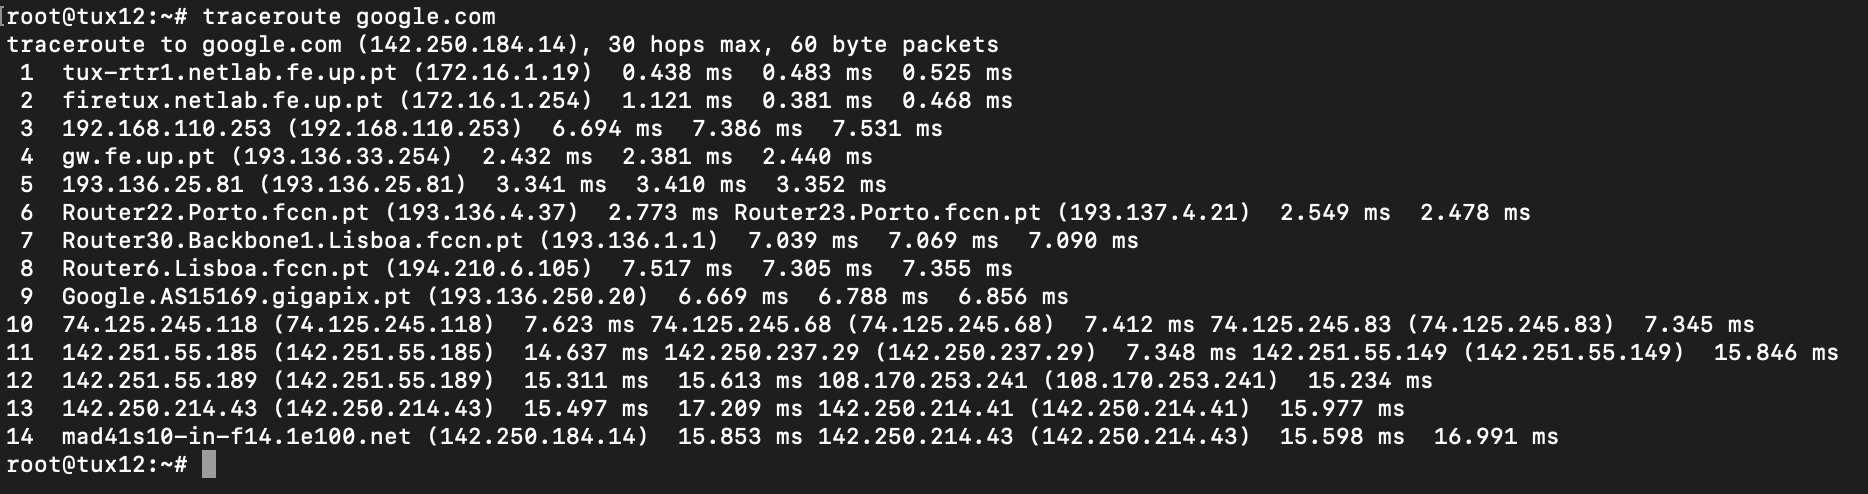
\includegraphics[width=.8\linewidth]{figs/setup/trace_1.png}
    \caption{Primeiro traceroute de google.com}
    \label{fig:traceroute_1}
\end{figure}

\begin{figure}
    \centering
    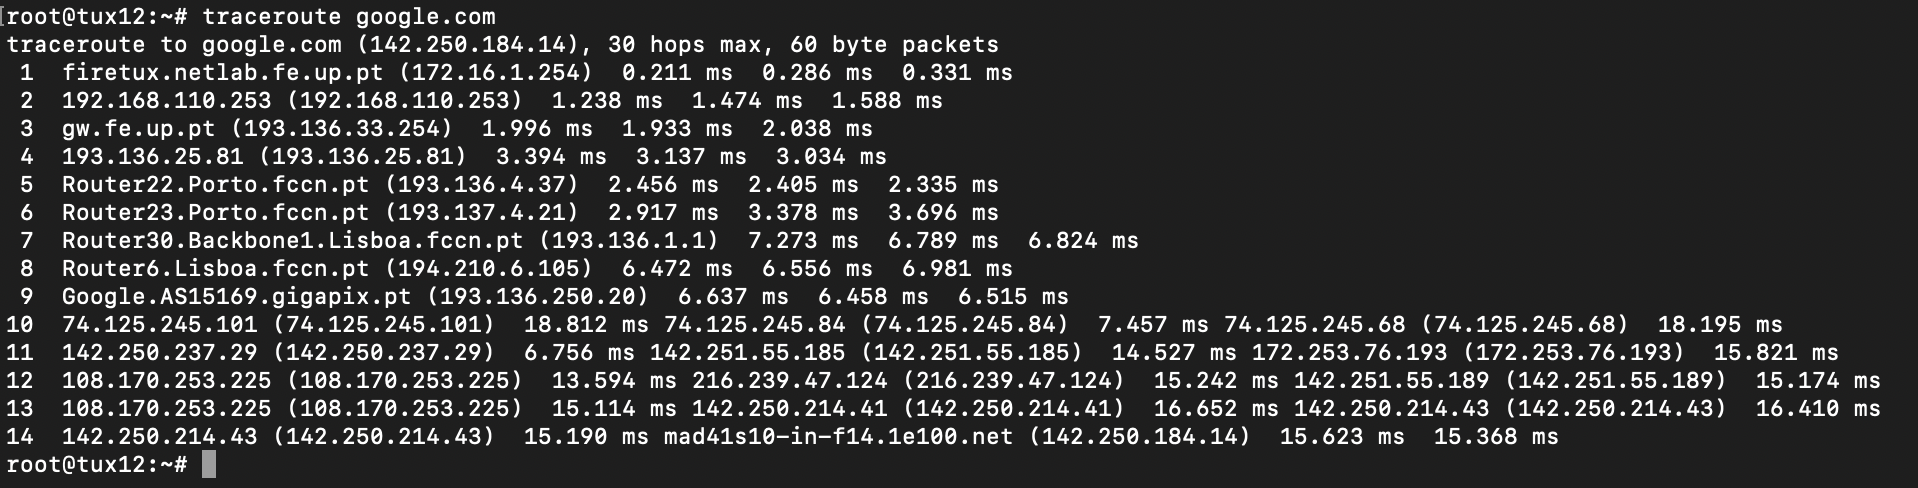
\includegraphics[width=.8\linewidth]{figs/setup/trace_2.png}
    \caption{Segundo traceroute de google.com}
    \label{fig:traceroute_2}
\end{figure}

Para voltar a forçar o caminho, é preciso apagar o routing cache, que é feito pelo próprio sistema periodicamente.

Em terceiro lugar, é preciso notar que o tráfego que vem de host externo \textbf{nunca} passa pelo router de bancada, a menos que seja direcionado para o mesmo.
Isto faz sentido dado que router de bancada não faz parte do caminho ótimo para os \textit{tux}.

Levanta-se então a nível do tráfego que nos é possível monitorizar. 
Todo o tráfego que é gerado no sentido \textit{Local->Remote} é monitorizado.
Tráfego \textit{Remote->Local / Local->Local} não é possível de observar.
Não podemos registar, por exemplo, acessos feitos ao nosso servidor FTP, ou emails enviados para o nosso servidor email.
A sincronização entre o NTP server e NTP client também não é analisado dado que é tráfego local.

Uma solução seria monitorizar o tráfego no switch, onde todo o tráfego passa obrigatoriamente. Teria por consequência ver-se no entanto também tráfego local de outras bancadas.

\subsection{Análise temporal}

O MRTG apresenta gráficos temporais do tráfego que passa pelo router, quer a entrar, quer a sair.
Devido ao período de tempo em que este esteve a monitorizar, só faz sentido apresentar o gráfico diário e semanal (Fig \ref{fig:mrtg_main}).

\begin{figure}
    \centering
    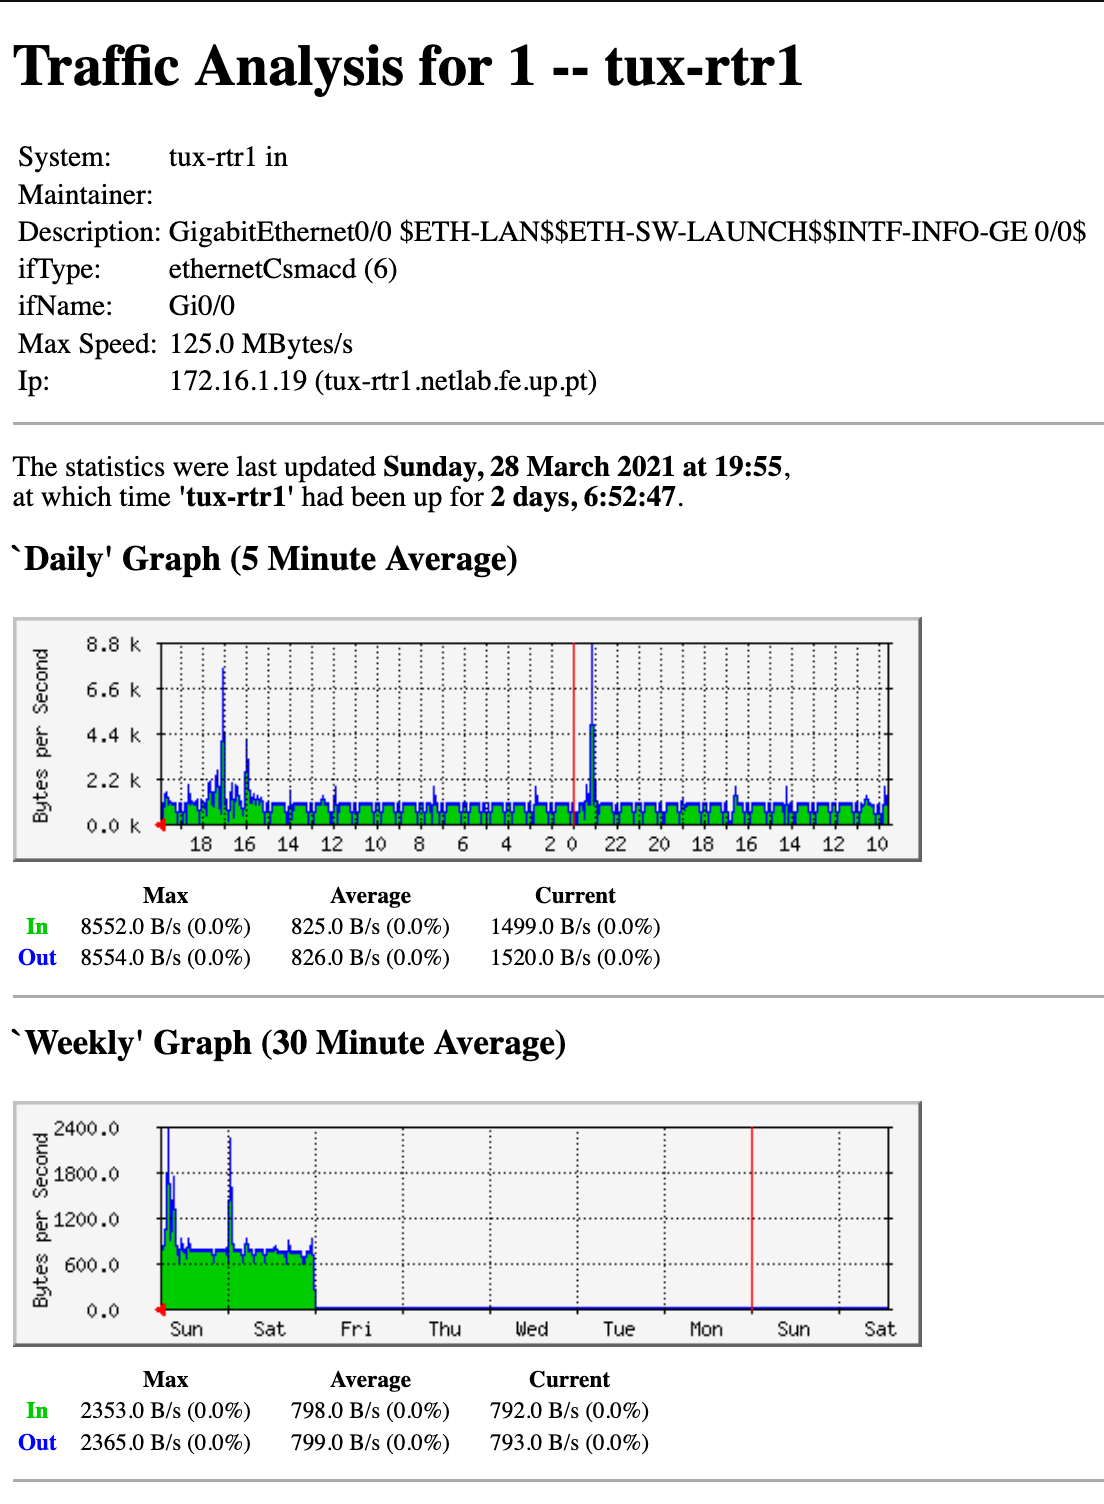
\includegraphics[width=.6\linewidth]{figs/setup/mrtg.png}
    \caption{Gráficos temporais do tráfego no router MRTG}
    \label{fig:mrtg_main}
\end{figure}

Como se pode observar, o gráfico é constante e apresenta um padrão a nível de picos que está relacionado com a temporização dos cronjobs.
Estes cronjobs fazem diferentes tarefas como enviar mails, fazer "digs" no DNS e aceder a servidores HTTP.
Os picos maiores devem-se a testes que estavam ser executados durante a configuração o sistema, como, por exemplo, pelo envio de muitos emails num curto espaço de tempo.

Constatamos também que o tráfego que entra é praticamos igual ao tráfego que sai. 
Isto deve-se ao facto de muito pouco tráfego ser destinado ao próprio router, funcionando este apenas como uma \textit{gate}.

\section{NTOP}

\subsection{Configuração}

O \textbf{NTOP} é uma ferramenta de monitorização de tráfico. Oferece uma versão comunitária grátis, assim como versões profissionais de subscrição.

O NTOP funciona escutando o tráfego num adaptador de rede, i.e., interface. No nosso caso, é utilizada a interface \textit{eth0}. É de notar que o NTOP consegue monitorizar várias interfaces ao mesmo tempo.
Desse modo, este foi configurado para escutar essa interface \cite{ntop}. A web-app do NTOP é acedida através do link \verb|172.16.1.12:3000| e depois é efetuado o login com os dados configurados.

\subsection{Análise global}

Dentro da web-app do NTOP, após selecionar a interface desejada, é-nos apresentada uma página inicial onde se pode observar resumo do tráfego nessa interface: (Fig \ref{fig:ntop_main})
\begin{itemize}
    \item Monitorização do tráfego em tempo real no canto superior esquerdo
    \item Tipo de tráfego, com 86\% a ser \textit{Local->Remote}.
    \item Total de tráfego registado pelo NTOP, com 205 MB enviado e 41.6 MB recebidos. Dado que estão a ser realizados acessos FTP externos, ocorre um aumento considerável do total de MB enviados pelo servidor.
\end{itemize}

\begin{figure}
    \centering
    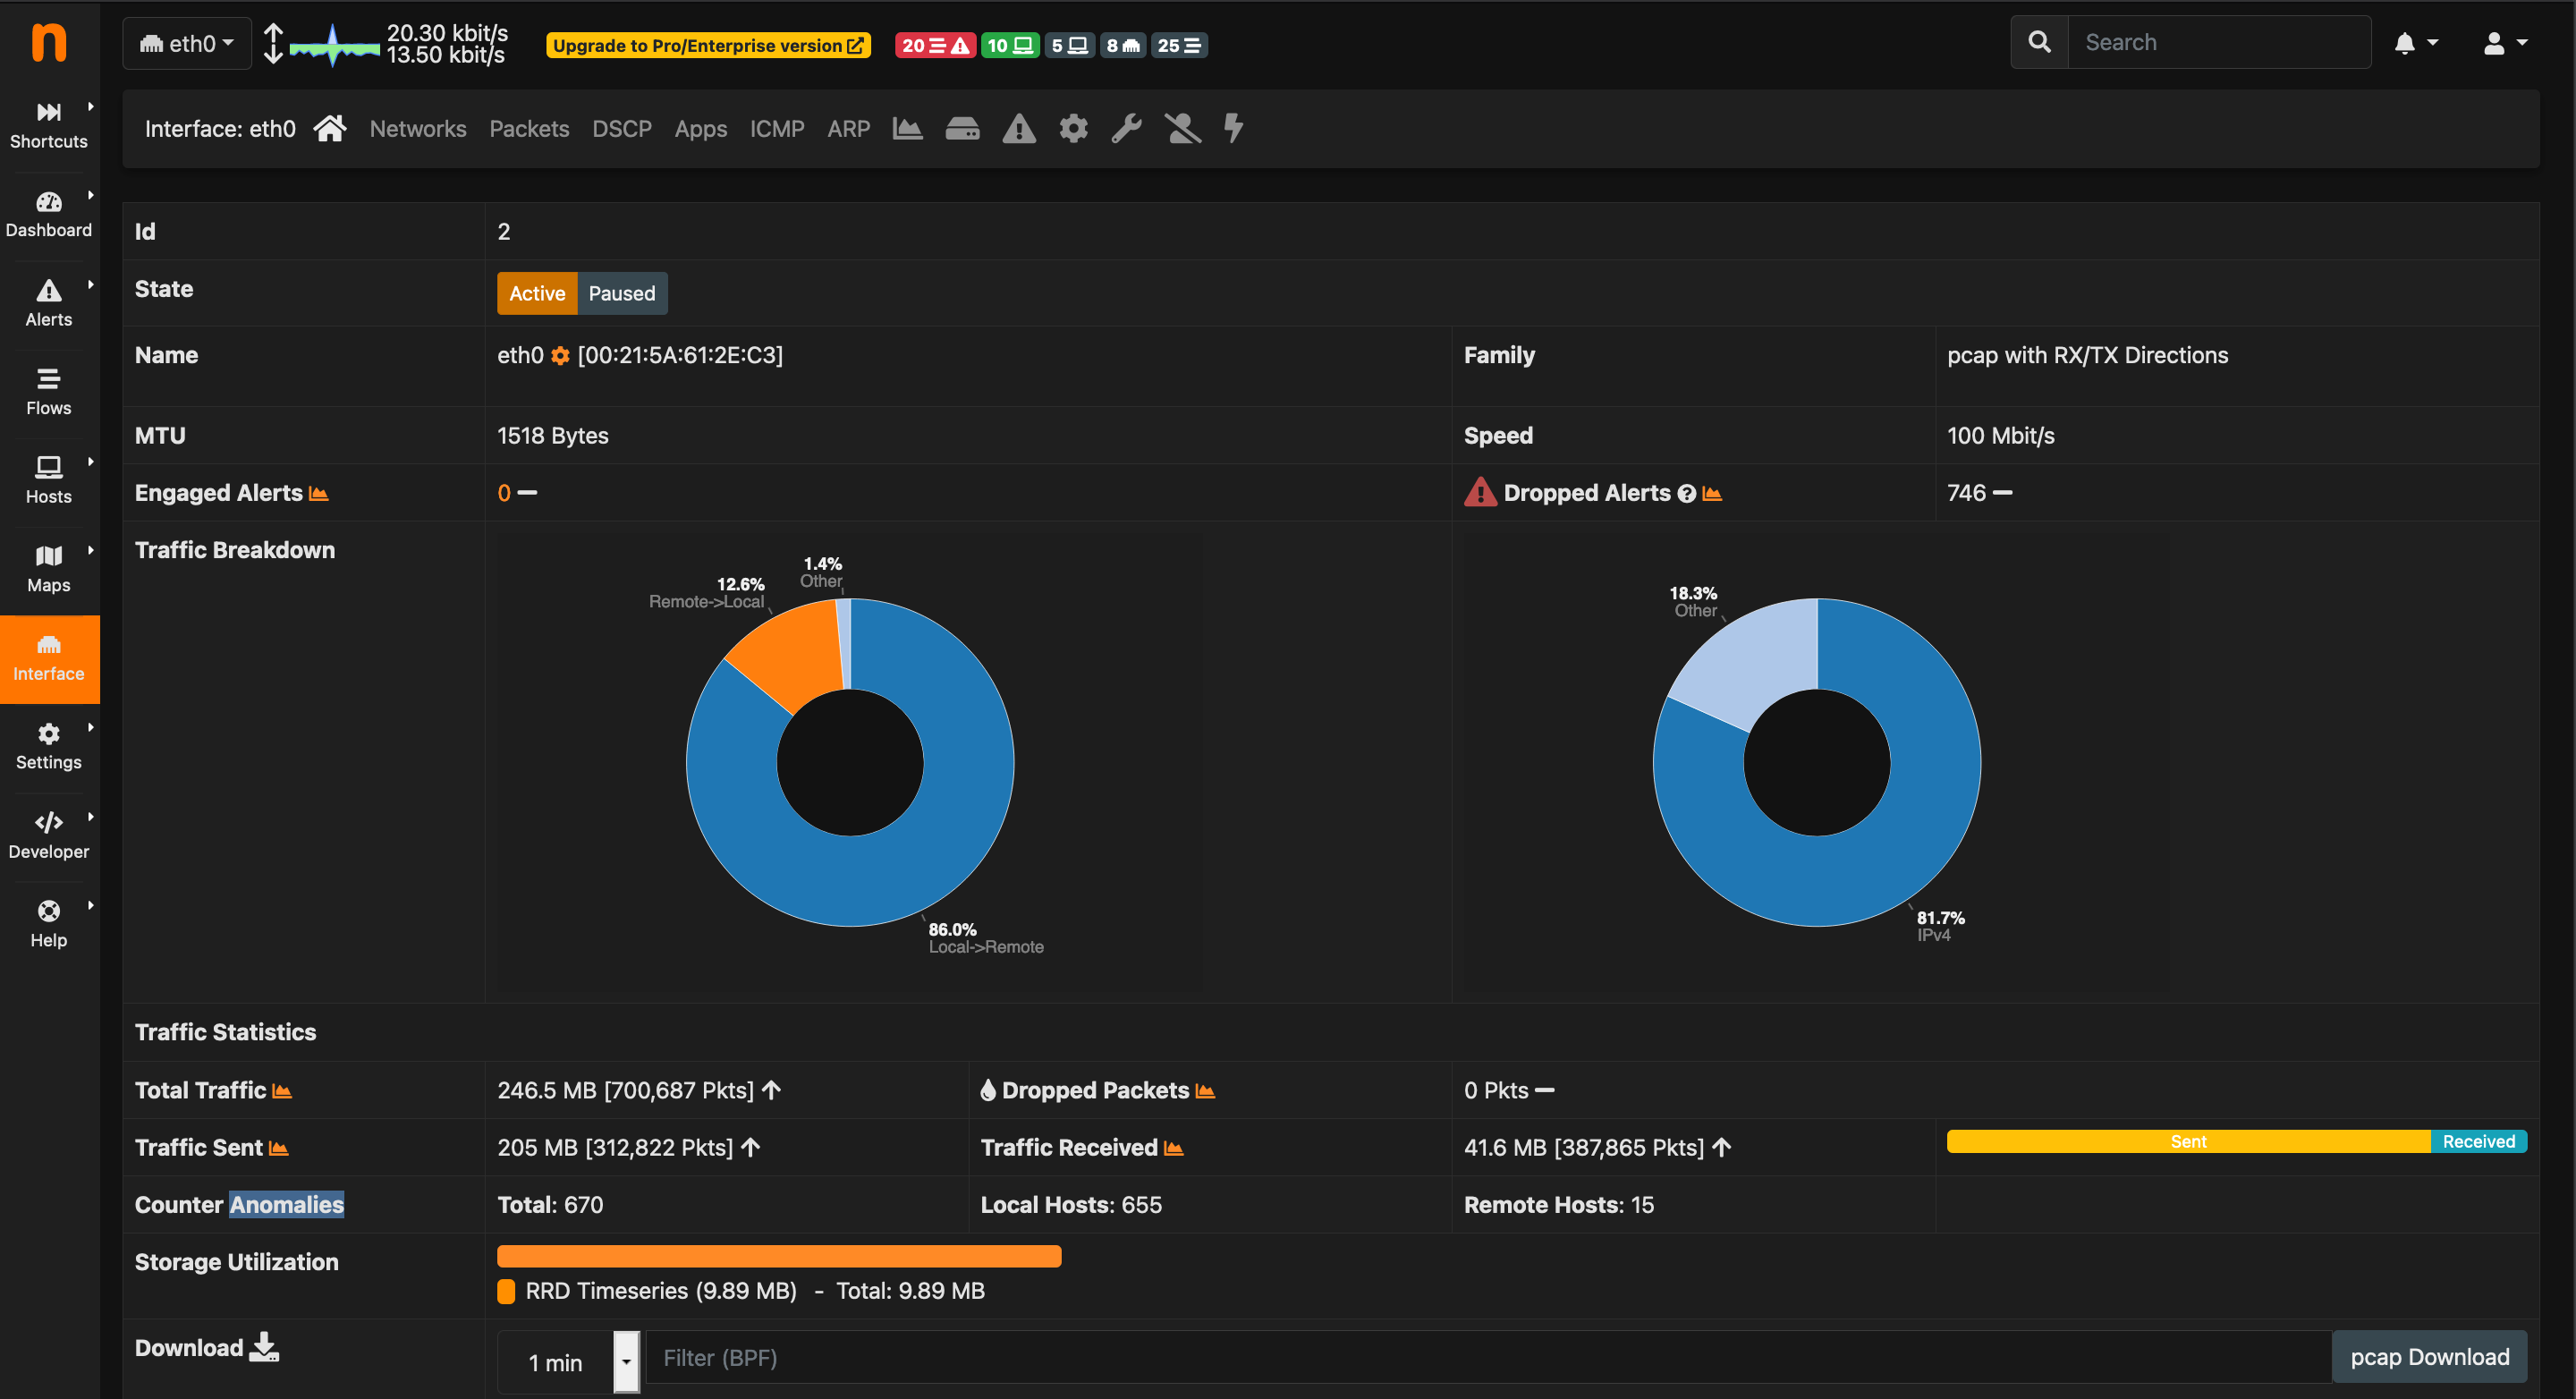
\includegraphics[width=.8\linewidth]{figs/setup/ntop_main.png}
    \caption{Main page da interface eth0}
    \label{fig:ntop_main}
\end{figure}

\subsection{Análise por tipologia}

Na tab "Apps", são apresentados 4 piecharts contendo a distribuição do tráfego por tipologia.
É apresentada uma avaliação total, assim como uma monitorização em tempo real (Fig \ref{fig:apps_charts}).

O \textit{FTP Data} corresponde a 52.4\% do tráfego, com o NTOP a representar 28.2\%.
Isto deve-se ao facto do NTOP gerar informação em realtime, que obriga a atualização constante da informação, gerando mais tráfego.
No momento em que foi tirado o print, não estava a ser detetado tráfego significativo de outros serviços, por isso o NTOP representa a maior fatia.

\begin{figure}
    \centering
    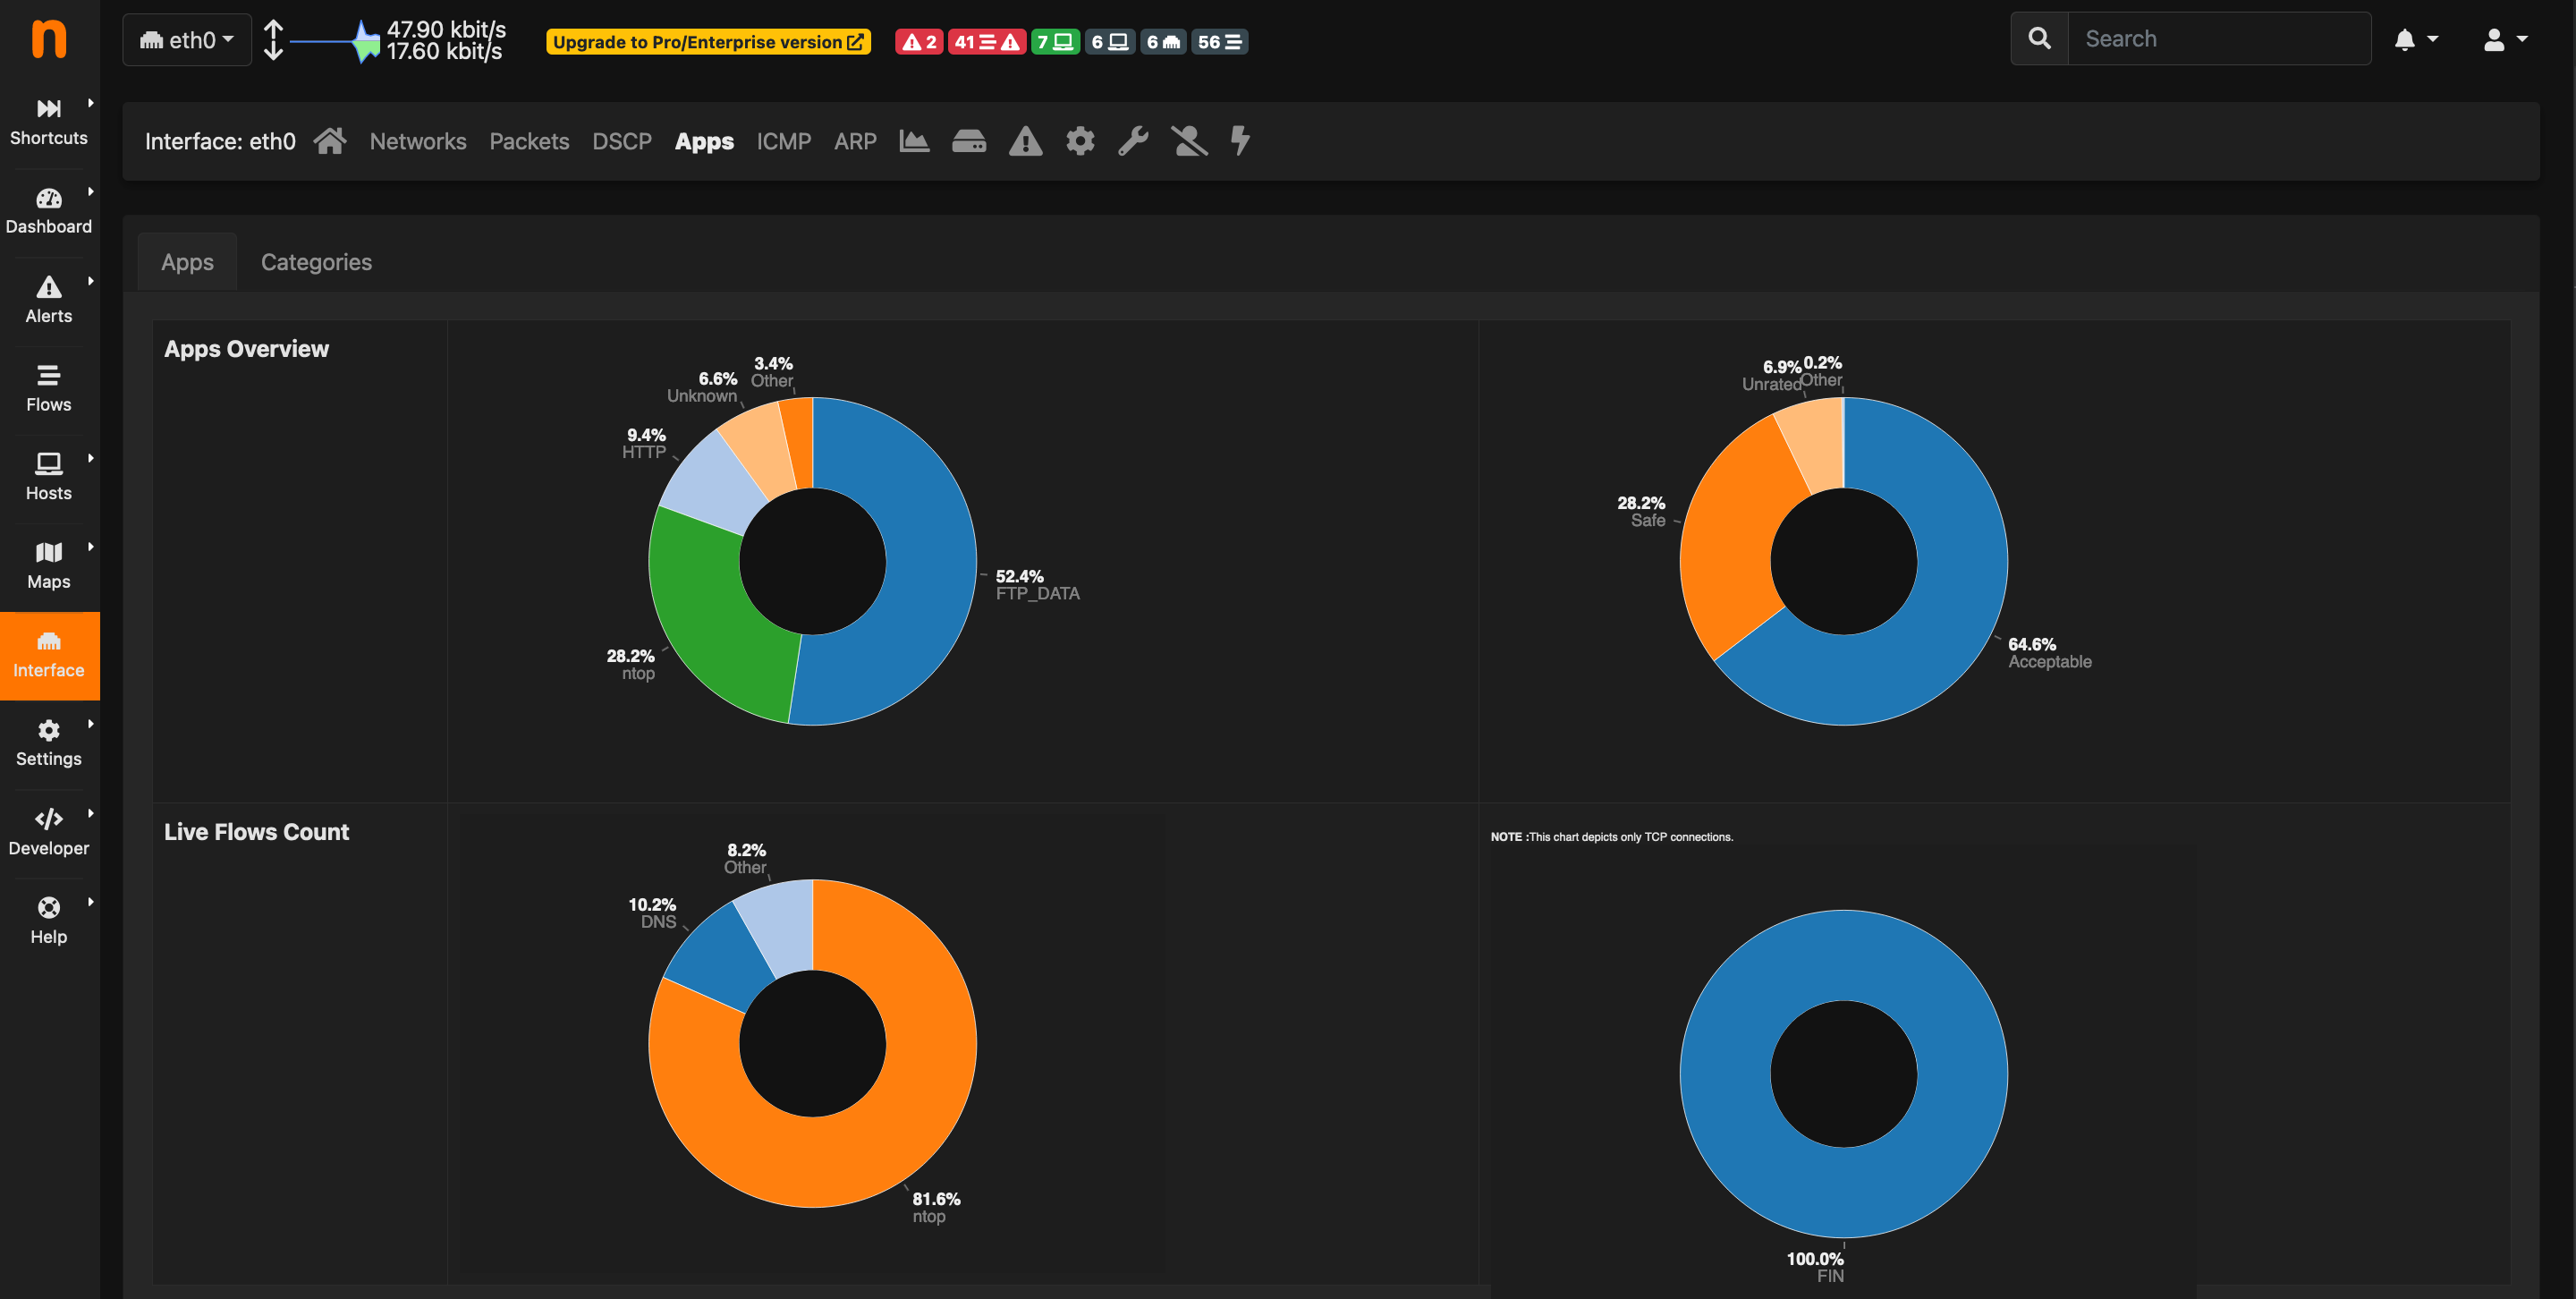
\includegraphics[width=.8\linewidth]{figs/setup/apps_charts.png}
    \caption{Piecharts da distribuição do tráfego por tipologia}
    \label{fig:apps_charts}
\end{figure}

Conseguimos também ver a distribuição total do tráfego em valores absolutos, onde podemos observar,
por exemplo, que o tráfego FTP representa a maior fatia de tráfego na interface (Fig \ref{fig:apps_table}).
Conseguimos também observar tráfego dos outros serviços instalados, nomeadamente DNS, HTTP, NTP e SMTP (Simple Mail Transfer Protocol).
O FTP estava a ser acedido para fazer download de um ficheiro de 250 Kb, pelo que gera mais tráfego.
O email por outro lado, era pequeno, pelo que gera menos tráfego.
Outros serviços são também detetados.


\begin{figure}
    \centering
    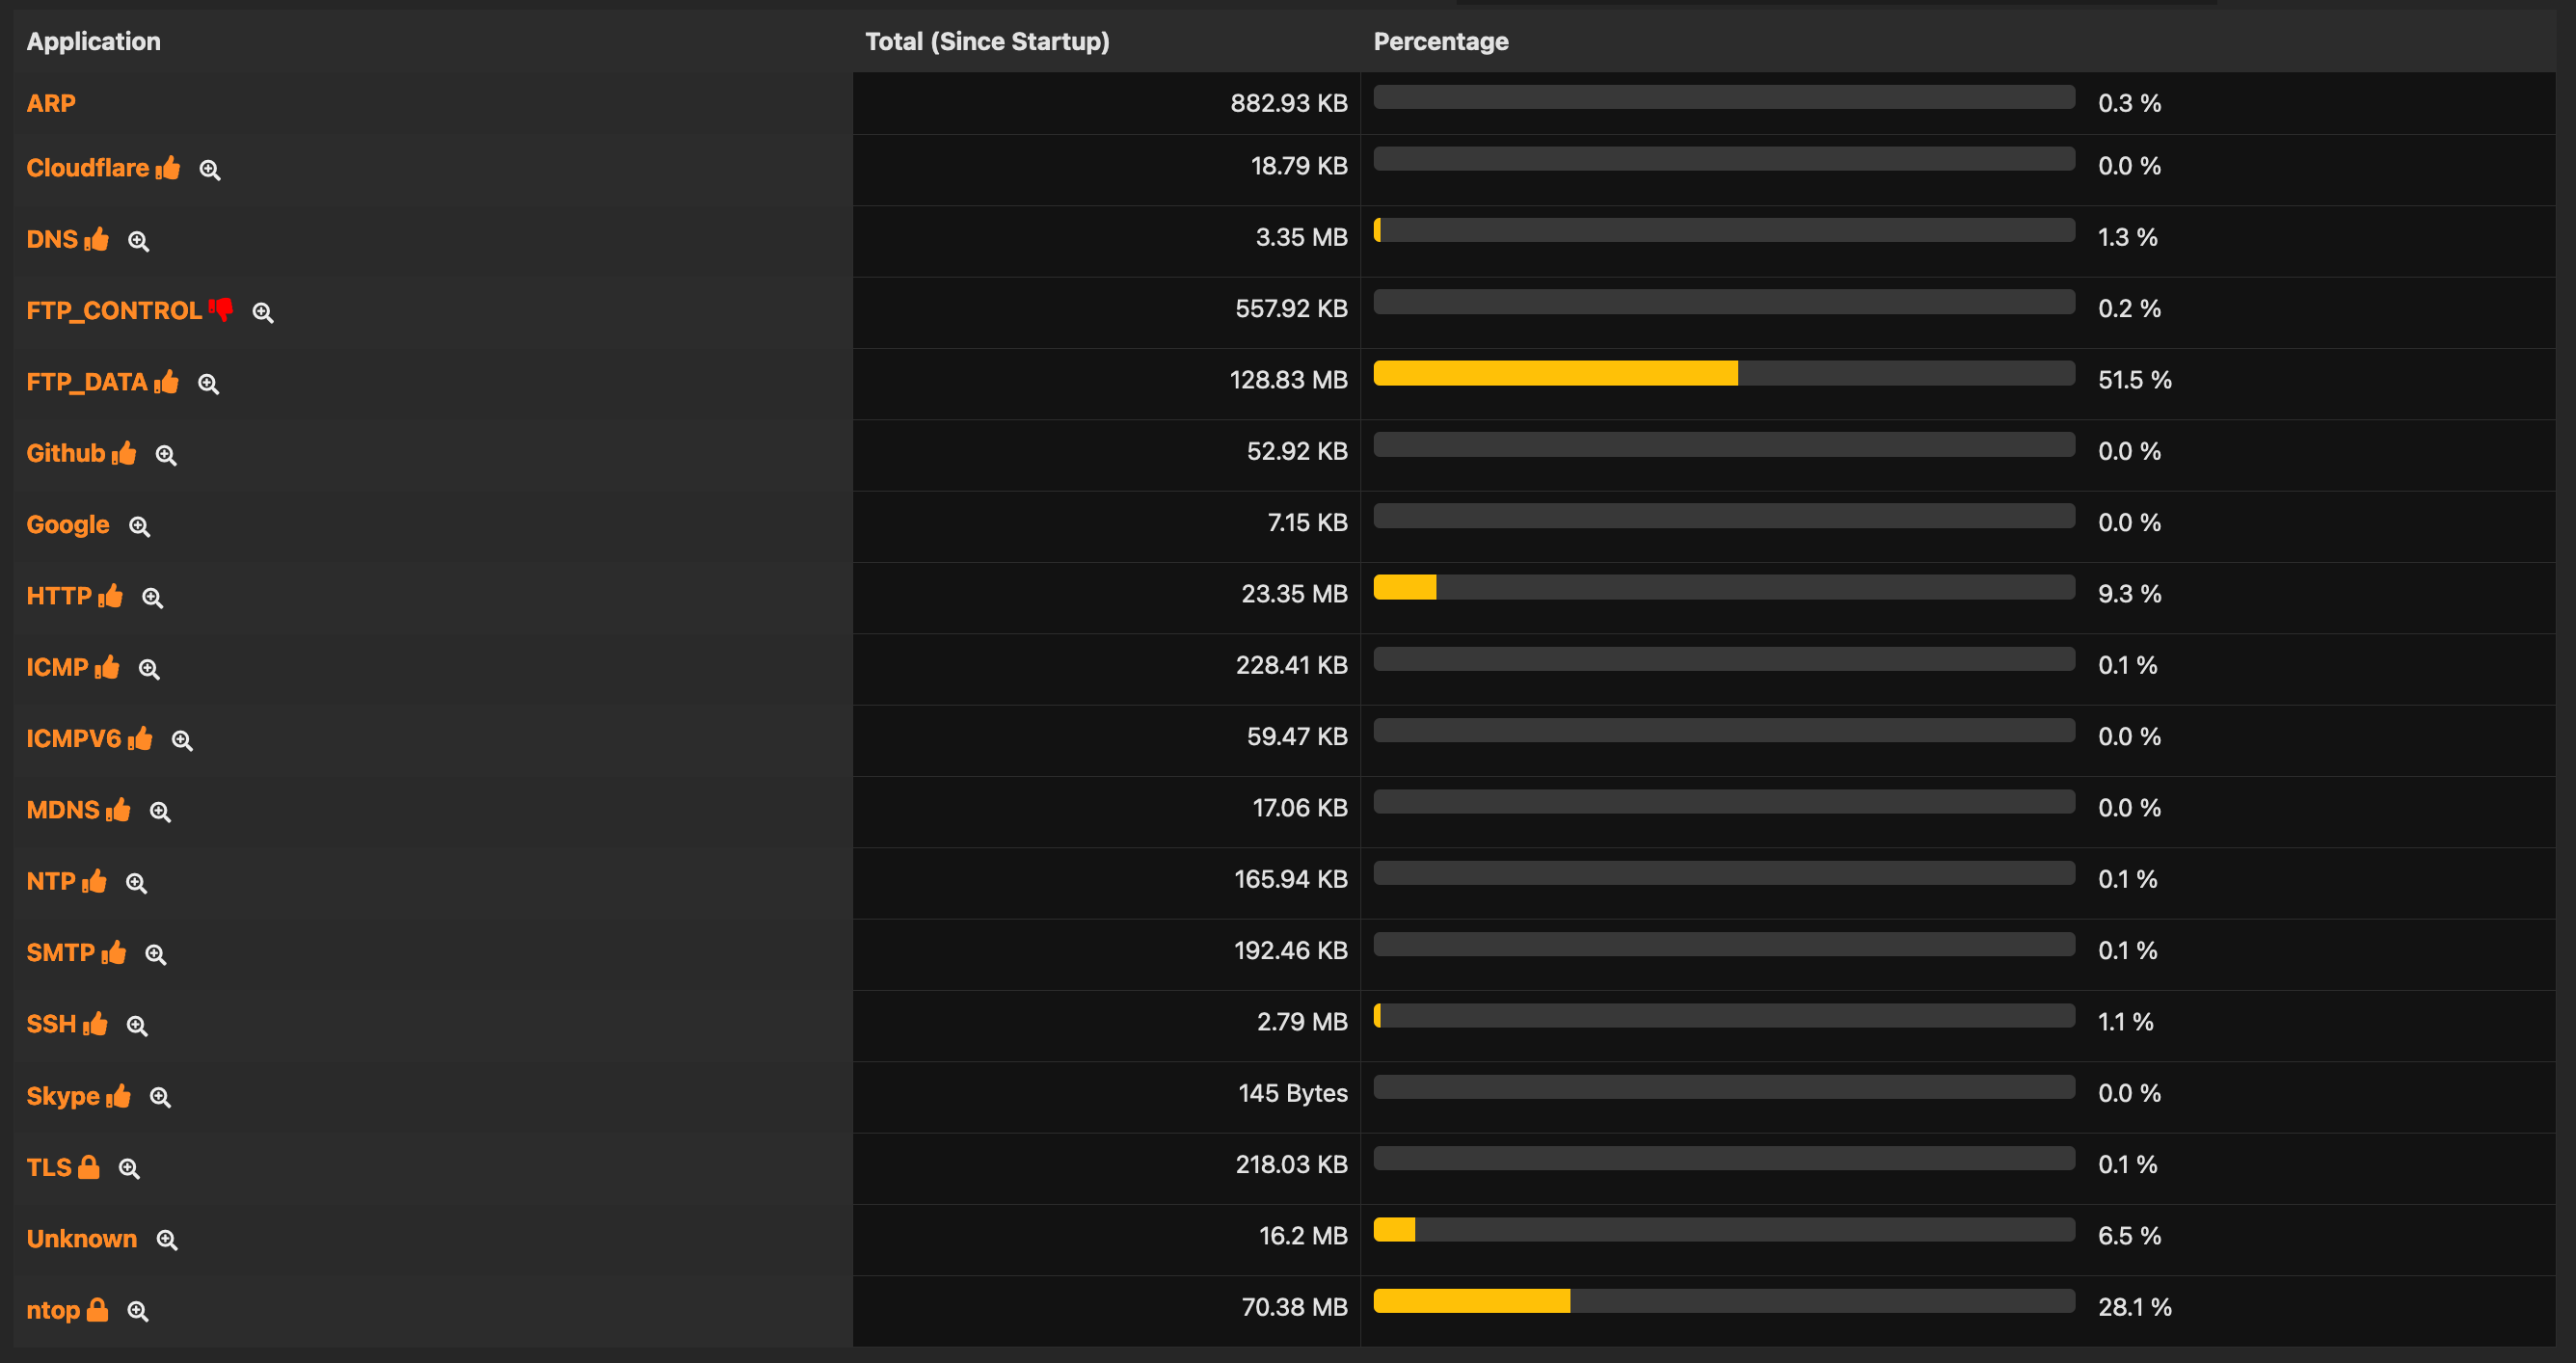
\includegraphics[width=.8\linewidth]{figs/setup/apps_tables.png}
    \caption{Distribuição do tráfego por tipologia}
    \label{fig:apps_table}
\end{figure}

\subsection{Análise temporal}

Tal como o MRTG, o NTOP também apresenta gráficos com a distribuição do tráfego a nível temporal.
Podemos observar diferentes intervalos temporais, como por exemplo, o horário (Fig \ref{fig:hourly}).
Podemos constatar neste gráfico vários picos periódicos de tráfego.
Estes correspondem, mais uma vez, aos pedidos FTP que geram muito mais tráfego que os restantes serviços.

\begin{figure}
    \centering
    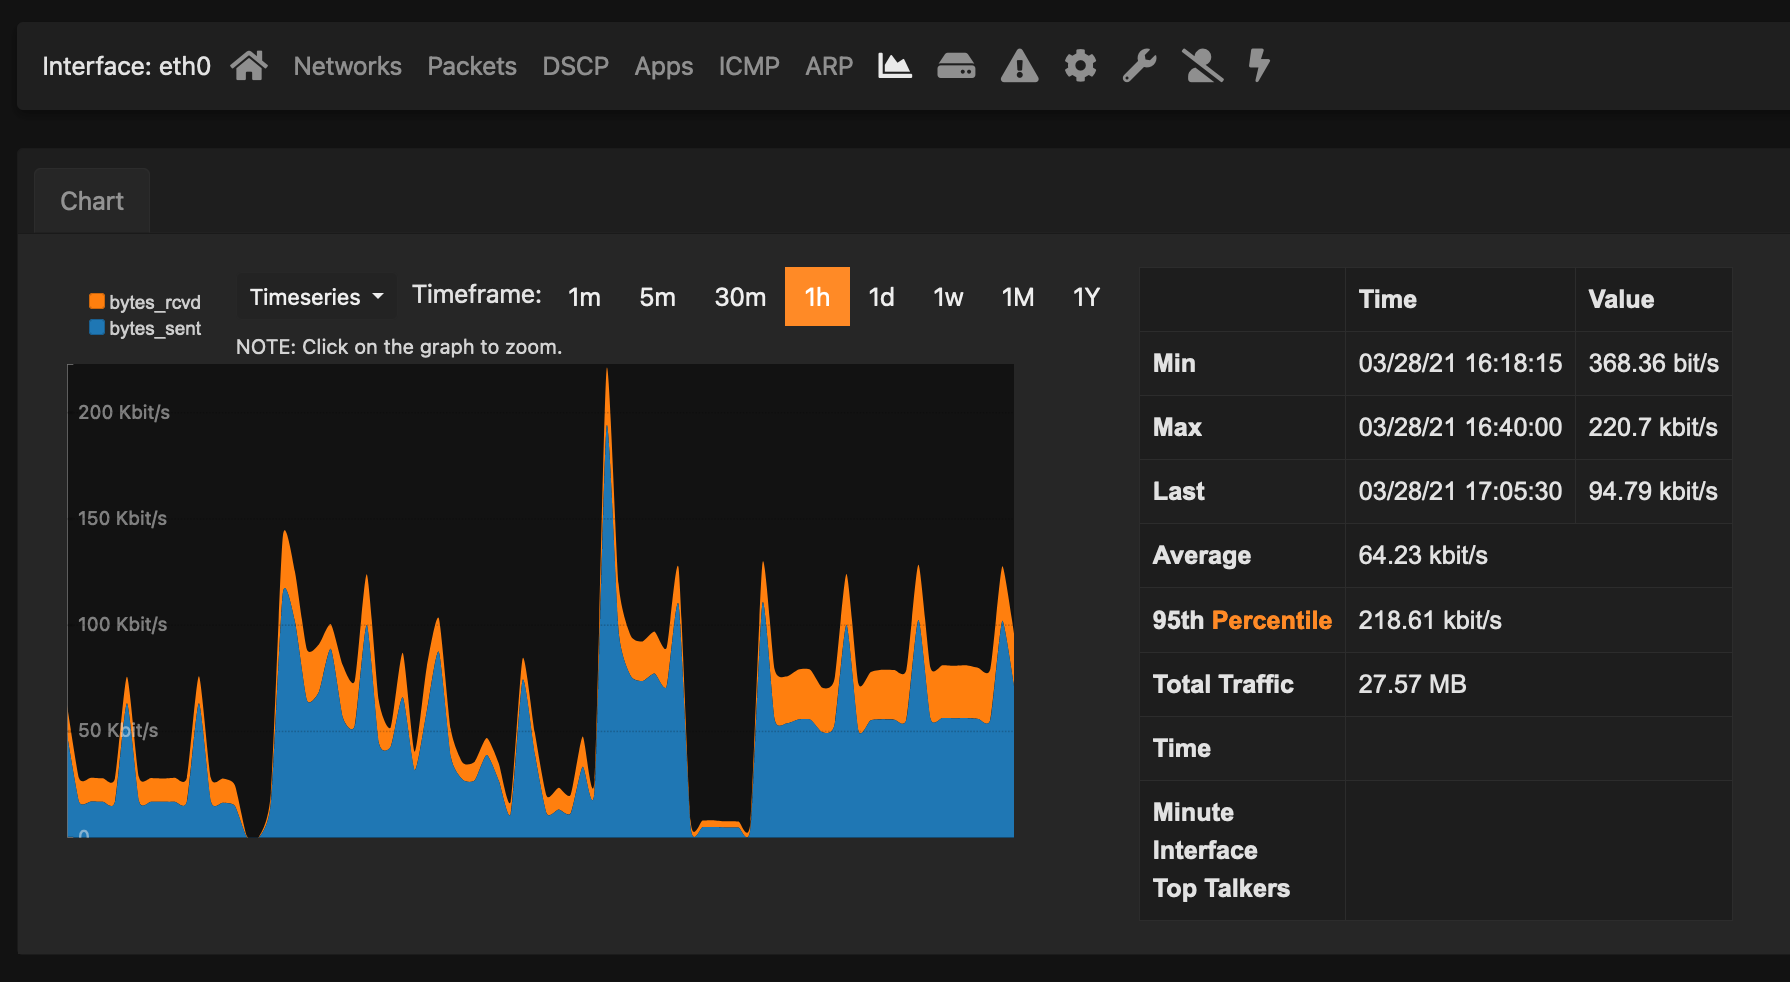
\includegraphics[width=.8\linewidth]{figs/setup/hourly.png}
    \caption{Análise horária do tráfego}
    \label{fig:hourly}
\end{figure}

\subsection{Análise dos Hosts}

O NTOP apresenta também uma lista de hosts que utilizaram a interface para enviar/receber tráfego (Fig \ref{fig:hosts}).
Esta lista é dinâmica e apresenta apenas os hosts ativos recentemente, mas é possível fazer uma pesquisa por qualquer host que tenha utilizado a interface.
Podemos constatar que o \textit{tux12} (172.16.1.12) gerou a maior parte do tráfego (243.74 MB).
Isto faz sentido dado que foi neste \textit{tux} que se instalaram todos os serviços.

\begin{figure}
    \centering
    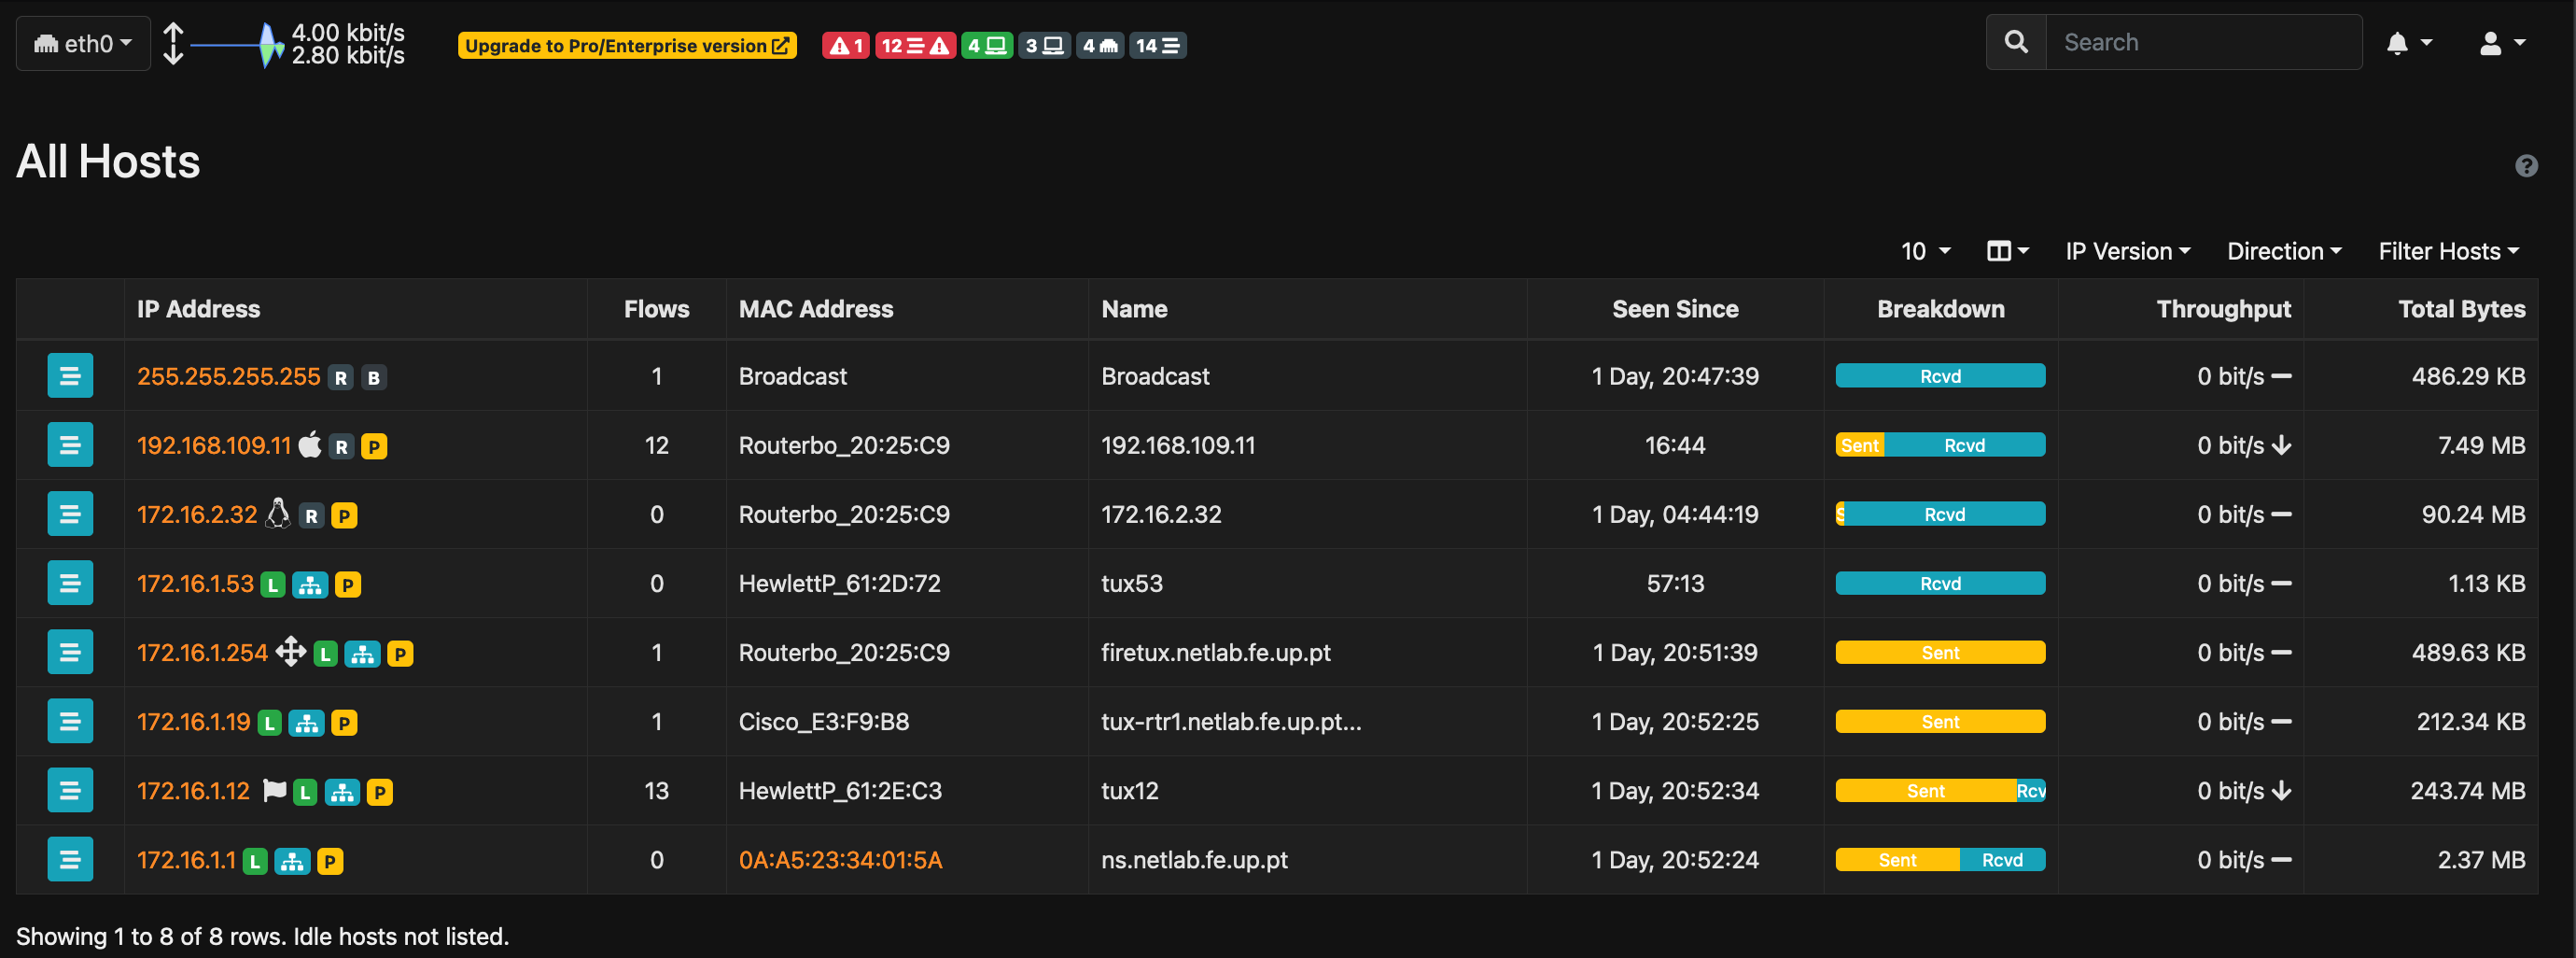
\includegraphics[width=.8\linewidth]{figs/setup/hosts.png}
    \caption{Lista dinâmica de hosts ativos}
    \label{fig:hosts}
\end{figure}

Também é possível fazer o mesmo tipos de análises que foram feitas para a interface, como a distribuição por tipologia e a distribuição temporal (Fig \ref{fig:hosts_apps}).

\begin{figure}
    \centering
    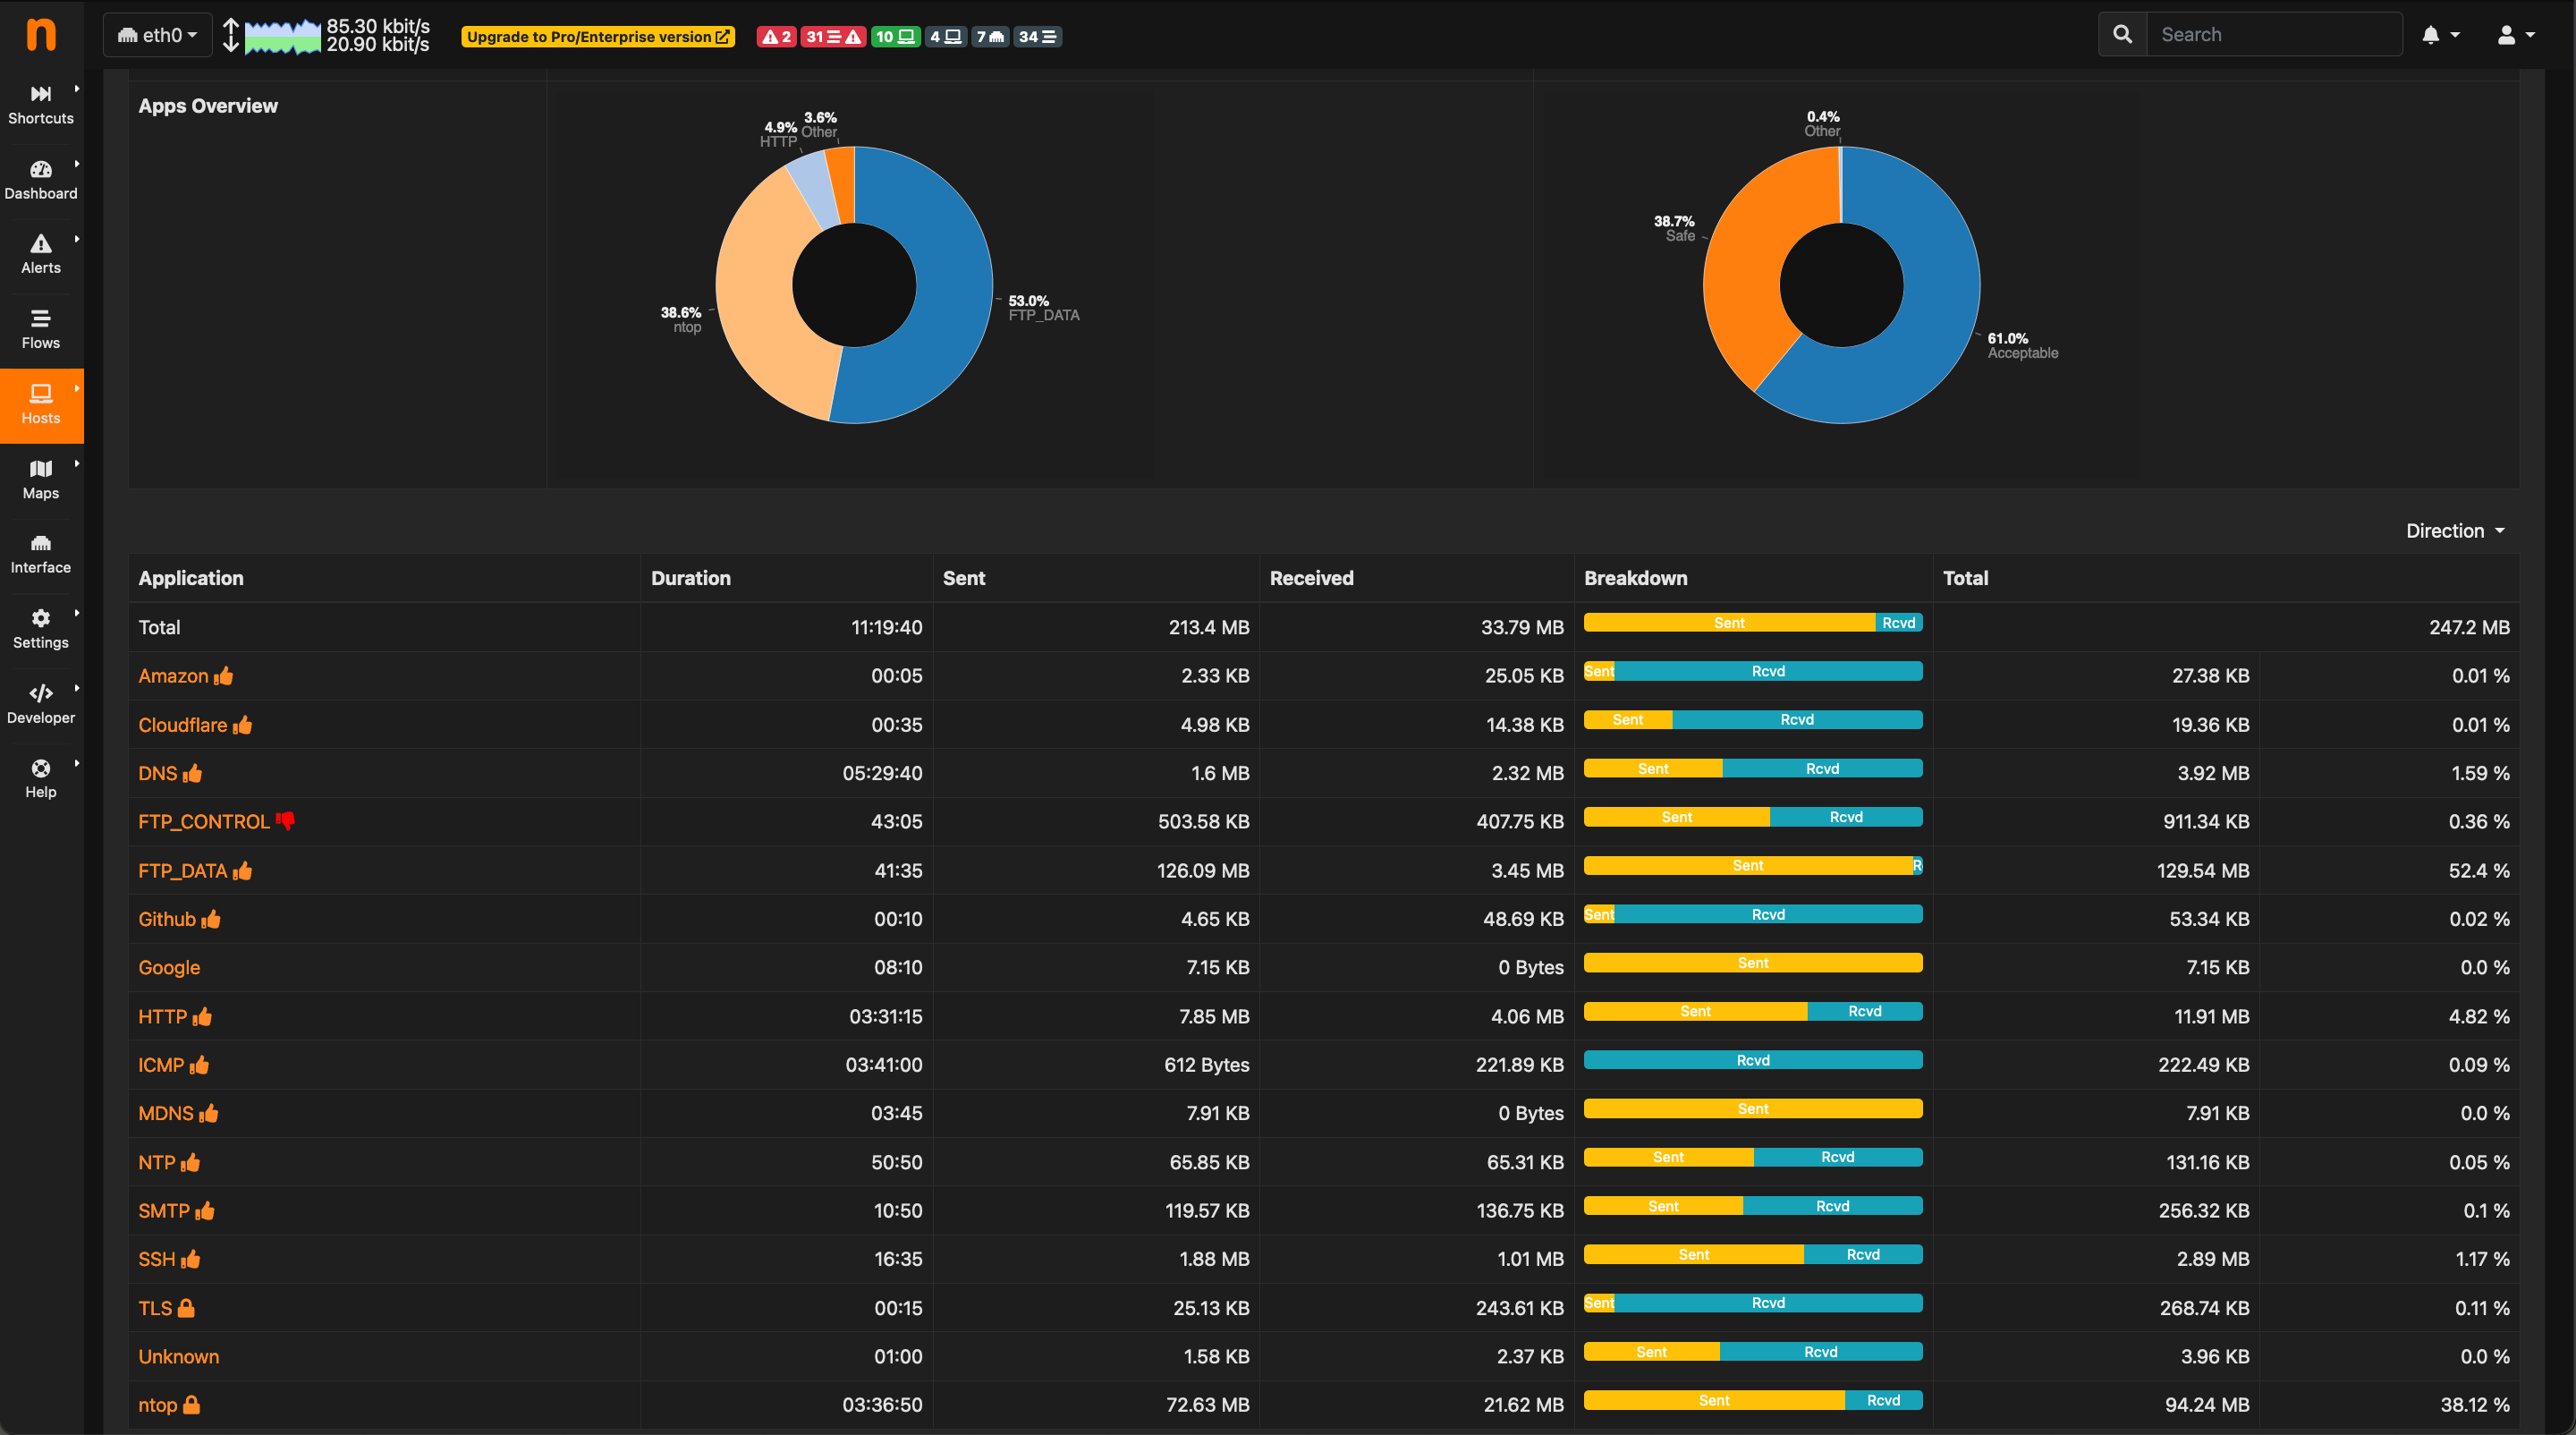
\includegraphics[width=.8\linewidth]{figs/setup/host_apps.png}
    \caption{Distribuição do tráfego por tipologia no tux12}
    \label{fig:hosts_apps}
\end{figure}

\subsection{Análise dos recursos do Sistema}

Além da análise do tráfego da interface, o NTOP apresenta também os recursos do sistema onde está instalado e o seu nível de utilização (Fig \ref{fig:system}).
Podemos observar gráficos de utilização do CPU do sistema para avaliar possíveis \textit{bottlenecks} a nível do hardware.
No nosso caso, os serviços instalados e a sua utilização não representam uma carga de utilização suficientemente grande para esta ferramenta ser útil neste projeto.

\begin{figure}
    \centering
    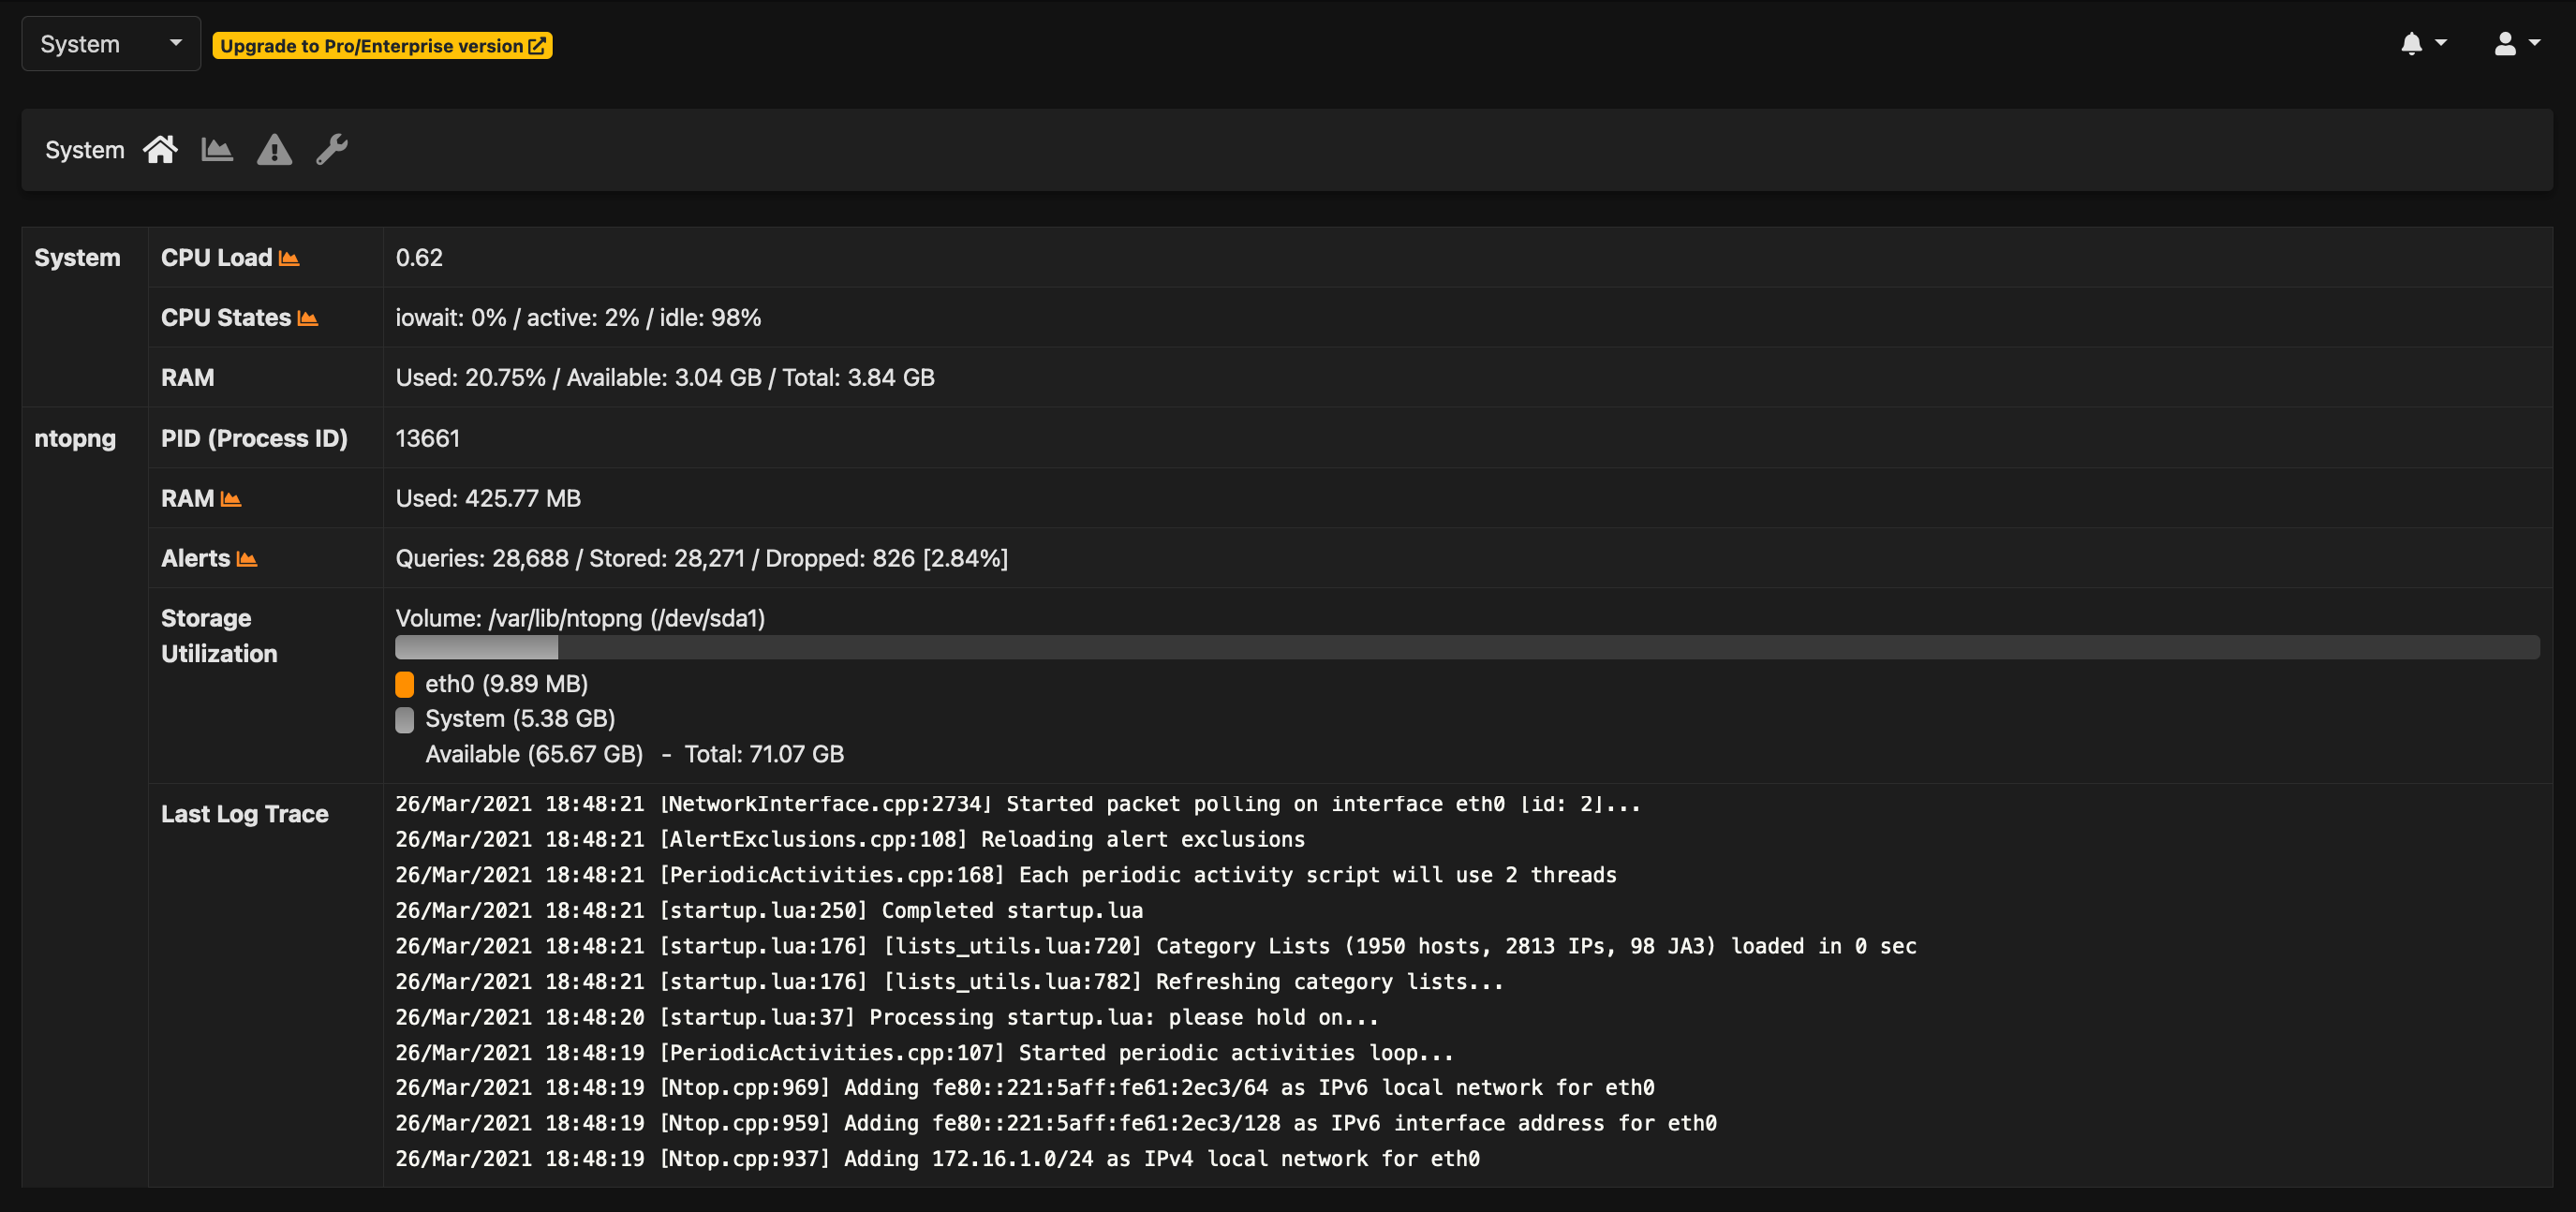
\includegraphics[width=.8\linewidth]{figs/setup/system.png}
    \caption{Utilização dos recursos do sistema}
    \label{fig:system}
\end{figure}

\section{Comparação}

Estas duas ferramentas e os resultados obtidos diferem em vários aspetos. Vamos analisar essas diferenças nesta secção.

\subsection{Monitorização de tráfego}

O NTOP, como mencionado anteriormente, regista todo o tráfego que usa a interface \textit{eth0}.
Esta interface é usada para praticamente todo tráfego, quer dentro da rede local quer externo.
Deste modo o NTOP é capaz de registar todo o tráfego dos serviços instalados no tux12.

O MRTG faz a monitorização do tráfego através do protocolo SNMP.
Ele foi configurado para monitorizar o router de bancada onde foi ativado o SNMP.
Pelas razões mencionadas na capítulo \ref{prop_rede}, o MRTG neste contexto não é capaz de ler todo o tráfego gerado pelos serviços, dado que nem todo o tráfego passa pelo router.
Desde modo, não é possível fazer uma análise total da utilização do nosso serviço com dois tipos de tráfego: \textit{Local->Local e Remote->Local}.

\subsection{User Interface}

O MRTG não faz distinção do tipo de tráfego.
De uma forma simples, apresenta gráficos com a evolução do tráfego total recebido e enviado ao longo do tempo.

O NTOP faz discriminação do tráfego, assim como da origem dele. Apresenta vários gráficos e tabelas onde podemos ver o tipo de tráfego, a sua origem, e a sua evolução ao longo do tempo.
Deste modo, podemos afirmar que o NTOP apresenta muita mais informação do que o MRTG.

Comparando os dois gráficos horários do NTOP (Fig \ref{fig:hourly}) e MRTG (Fig \ref{fig:mrtg_main}), pode-se observar que no MRTG não estão presentes os picos de tráfego em 100kB que vemos no NTOP.
Isto deve-se ao facto do tráfego FTP não estar a ser monitorizado. Estão a ser realizados acessos FTP do tipo \textit{Remote->Local}, um tipo de tráfego que não passa pelo router de bancada.
Para se poder observar tráfego FTP, seria necessário fazer ligações a servidores FTP da outra sala.
Isto não foi possível realizar em tempo útil, pois à data da recolha dos dados, não havia servidores FTP na outra sala disponíveis para este teste.

\subsection{Use Cases}
O NTOP provou ser a melhor ferramenta neste contexto. No entanto, não regista o tráfego utilizado por outras interfaces de outros \textit{tux}s.
Como na nossa configuração, todos os serviços estavam instados no \textit{tux12}, isto não foi um problema.

O MRTG é mais útil para monitorizar o tráfego de um servidor. Se estivéssemos a ler o switch, iríamos conseguir ver todo o tráfego \textit{Local->Local / Remote->Local / Local->Remote}.
Isto seria mais útil, sendo que estaríamos a ver todo o tráfego gerado por todos os hosts dentro da sala I321.

Ao ler router \textbf{firetux}, não íamos conseguir ver tráfego local.


